%%%%%%%%%%%%%%%%%%%%%%%%%%%%%%%%%%%%%%%%%
% Jacobs Landscape Poster
% LaTeX Template
% Version 1.1 (14/06/14)
%
% Created by:
% Computational Physics and Biophysics Group, Jacobs University
% https://teamwork.jacobs-university.de:8443/confluence/display/CoPandBiG/LaTeX+Poster
% 
% Further modified by:
% Nathaniel Johnston (nathaniel@njohnston.ca)
%
% This template has been downloaded from:
% http://www.LaTeXTemplates.com
%
% License:
% CC BY-NC-SA 3.0 (http://creativecommons.org/licenses/by-nc-sa/3.0/)
%
%%%%%%%%%%%%%%%%%%%%%%%%%%%%%%%%%%%%%%%%%

%----------------------------------------------------------------------------------------
%	PACKAGES AND OTHER DOCUMENT CONFIGURATIONS
%----------------------------------------------------------------------------------------

\documentclass[final]{beamer}

\usepackage[scale=1.24]{beamerposter} % Use the beamerposter package for laying out the poster

\usetheme{confposter} % Use the confposter theme supplied with this template

\setbeamercolor{block title}{fg=ngreen,bg=white} % Colors of the block titles
\setbeamercolor{block body}{fg=black,bg=white} % Colors of the body of blocks
\setbeamercolor{block alerted title}{fg=white,bg=dblue!70} % Colors of the highlighted block titles
\setbeamercolor{block alerted body}{fg=black,bg=dblue!10} % Colors of the body of highlighted blocks
% Many more colors are available for use in beamerthemeconfposter.sty

%-----------------------------------------------------------
% Define the column widths and overall poster size
% To set effective sepwid, onecolwid and twocolwid values, first choose how many columns you want and how much separation you want between columns
% In this template, the separation width chosen is 0.024 of the paper width and a 4-column layout
% onecolwid should therefore be (1-(# of columns+1)*sepwid)/# of columns e.g. (1-(4+1)*0.024)/4 = 0.22
% Set twocolwid to be (2*onecolwid)+sepwid = 0.464
% Set threecolwid to be (3*onecolwid)+2*sepwid = 0.708

\newlength{\sepwid}
\newlength{\onecolwid}
\newlength{\twocolwid}
\newlength{\threecolwid}
\setlength{\paperwidth}{1189mm} % A0 width: 46.8in
\setlength{\paperheight}{841mm} % A0 height: 33.1in
\setlength{\sepwid}{0.02\paperwidth} % Separation width (white space) between columns
\setlength{\onecolwid}{0.225\paperwidth} % Width of one column
\setlength{\twocolwid}{0.47\paperwidth} % Width of two columns
\setlength{\threecolwid}{0.715\paperwidth} % Width of three columns
\setlength{\topmargin}{-25mm} % Reduce the top margin size

\addtobeamertemplate{block end}{}{\vspace*{2ex}} % White space under blocks
\addtobeamertemplate{block alerted end}{}{\vspace*{2ex}} % White space under highlighted (alert) blocks

\setlength{\belowcaptionskip}{2ex} % White space under figures
\setlength\belowdisplayshortskip{2ex} % White space under equations

\usepackage{graphicx}  % Required for including images

\usepackage{booktabs} % Top and bottom rules for tables

\usepackage{amsmath,amssymb,amsfonts,anyfontsize}
\usepackage{algorithmic}
\usepackage{textcomp}
\usepackage{xcolor}
\usepackage{stfloats}
\usepackage[caption=false, font=footnotesize]{subfig}
\usepackage{arydshln}
\usepackage{slashbox}

\title{{\fontsize{86}{60}\selectfont Estimating Subgraph Generation Models to Understand Large Network Formation}} % Poster title
\author{\parbox{.18\textwidth}{\hfill \strut Laurens Bogaardt\hspace{8mm}\strut} \parbox{.18\textwidth}{\strut\hspace{6mm} Frank W. Takes\strut}}
\institute{
\parbox{.32\textwidth}{\vspace{-32mm} \centering 
\includegraphics[height=4cm]{NLeSc.png}}
\parbox{.16\textwidth}{\hfill \strut Netherlands eScience Center\hspace{6mm}\strut}
\parbox{.16\textwidth}{\strut\hspace{8mm} University of Amsterdam\strut}
\parbox{.32\textwidth}{\vspace{-32mm} \centering 
\includegraphics[height=4cm]{UvA.png}}\vspace{-6mm}
}
\usebackgroundtemplate{\includegraphics[height=\paperheight, width=\paperwidth]{NLeScBackground.jpg}}

\begin{document}

\begin{frame}[t] % The whole poster is enclosed in one beamer frame

\begin{columns}[t] % The whole poster consists of three major columns, the second of which is split into two columns twice - the [t] option aligns each column's content to the top

\begin{column}{\sepwid}\end{column} % Empty spacer column

\begin{column}{\threecolwid} % Begin a column which is two columns wide (column 2)

\begin{columns}[t,totalwidth=\threecolwid] % Split up the two columns wide column

\begin{column}{\onecolwid}\vspace{-.5in} % The first column

\begin{alertblock}{Abstract}

Recently, a new network formation model was proposed. The current research looks into a method to estimate the parameters of this model based on the subgraph census.\\

\end{alertblock}

\begin{block}{Introduction}

Social scientists often aim to understand the incentives and mechanisms which result in large scale socio-economic structures. Key to this is network formation analysis. However, large datasets are not uncommon, leading to a computational challenge. For example, political scientists interested in global networks of corporate control may need to analyse millions of companies to answer their questions~\cite{Takes2016,Fennema2018}.

\end{block}

\begin{block}{ERGM}

The Exponential Random Graph Model (ERGM) is a frequently used network formation model. Unfortunately, it suffers from two fundamental flaws. Firstly, its parameter estimates are inconsistent~\cite{Shalizi2013,Chatterjee2013}. Secondly, it does not scale well~\cite{Bhamidi2011}. Recently, an alternative network formation model was suggested: the Subgraph Generation Model (SUGM)~\cite{Chandrasekhar2014,Chandrasekhar2015,Chandrasekhar2016}.

\end{block}

\end{column} % End of the first column

\begin{column}{\sepwid}\end{column} % Empty spacer column

\begin{column}{\onecolwid}\vspace{-.6in} % The first column within column 2 (column 2.1)

\begin{block}{SUGM}

A SUGM is defined by a set of $l$ small subgraphs, such as links, triangles or stars, each with corresponding probabilities. For each subgraph $i$ of $m_{i}$ nodes, the $n$ nodes of the entire network are grouped into all possible subsets of $m_{i}$ nodes. Then, each of these subsets receives the subgraph $i$ with probability $1-p_{i}$ or remains empty with probability $p_{i}$.

The observed network, depicted in Fig.~\ref{fig:Figure01}, is the union of all these subgraphs, depicted in Fig.~\ref{fig:Figure02}. The various generated subgraphs may have some overlapping edges. Multiple neighbouring subgraphs may incidentally form additional structures such as triangles or squares.

\end{block}

\setbeamertemplate{block begin}[notitle]
\begin{block}

\begin{figure}
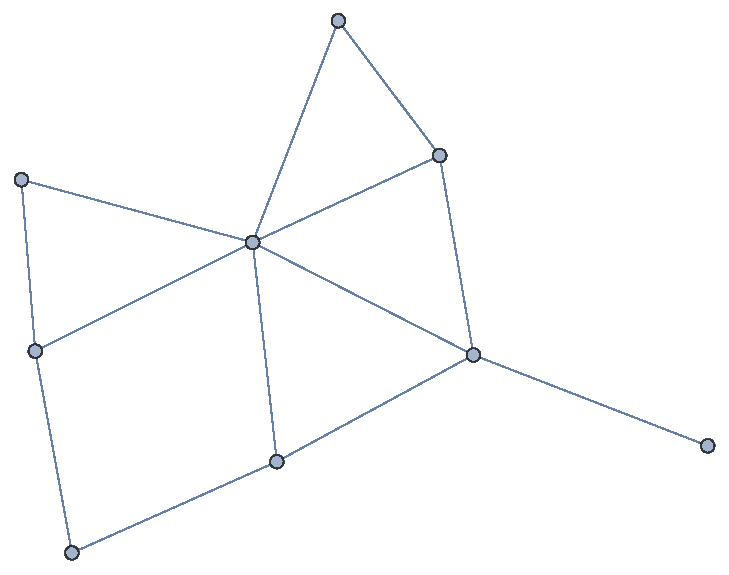
\includegraphics[width=0.8\linewidth]{../Figure02_1.pdf}
\caption{\hspace{3mm}The observed network is the union of randomly generated subgraph.}
\label{fig:Figure01}
\end{figure}

\end{block}
\setbeamertemplate{block begin}[default]

\end{column} % End of column 2.1

\begin{column}{\sepwid}\end{column} % Empty spacer column

\begin{column}{\onecolwid}\vspace{-.6in} % The second column within column 2 (column 2.2)

\begin{block}{Estimation}

The original articles describing SUGM contain two methods to estimate the parameters of the model. The current research suggests a third, more intuitive method based on the subgraph census. In a $k$-subgraph census, a network of $n$ nodes is grouped into all possible subsets of $k$ nodes, which are then tallied according to their isomorphism class~\cite{Davis1972,Holland1970,Holland1976}.

The table below contains the probabilities of observing any of the possible triads for three different generation models. In general, each of the $r$ counts of the census $x_{j}$, together with the probability functions $f_{j}(\hat{p}_{1},\cdots,\hat{p}_{l})$, enter into the multinomial ...

\end{block}

\setbeamertemplate{block begin}[notitle]
\begin{block}

\begin{figure}
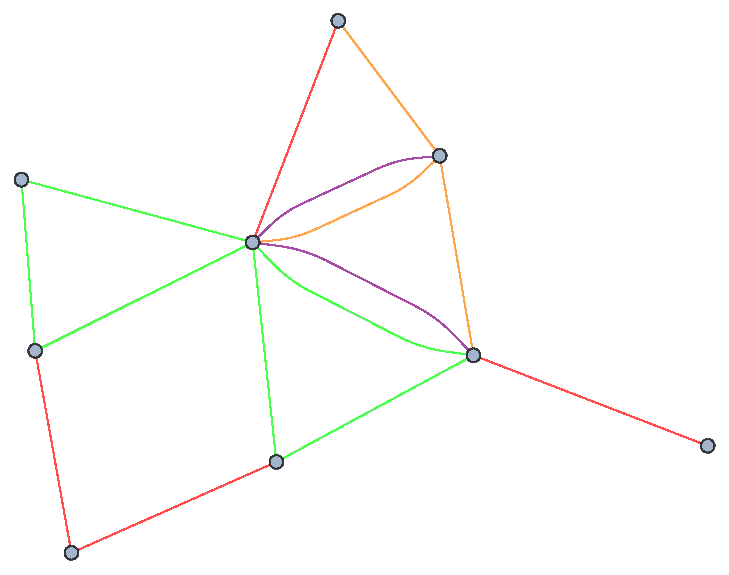
\includegraphics[width=0.8\linewidth]{../Figure02_2.pdf}
\caption{\hspace{3mm}Randomly generated links (red), 2-paths (purple), triangles (green) and 3-stars (yellow).}
\label{fig:Figure02}
\end{figure}

\end{block}
\setbeamertemplate{block begin}[default]

\end{column} % End of column 2.2

\end{columns} % End of the split of column 2 - any content after this will now take up 2 columns width

\begin{alertblock}{Probabilities in the Subgraph Census}

\begin{table}[b]
\def\arraystretch{1.5}
\setlength\tabcolsep{12mm}
\begin{center}
\begin{tabular}{c|c:c:c:c}
\backslashbox{\textbf{Model}}{\textbf{Types}}&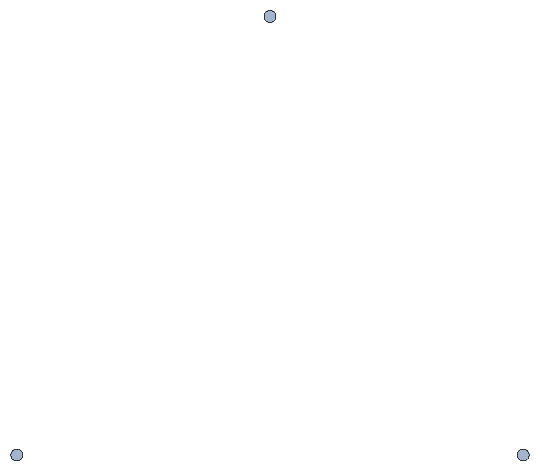
\includegraphics[  scale=1.5]{../Figure03_1.pdf}&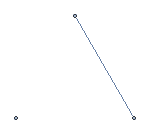
\includegraphics[  scale=1.5]{../Figure03_2.pdf}&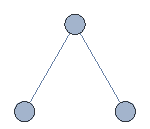
\includegraphics[  scale=1.5]{../Figure03_3.pdf}&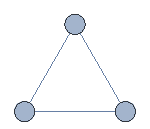
\includegraphics[  scale=1.5]{../Figure03_4.pdf}\\
\hline
Links & $p_{L}^{3}$ & $3 \, p_{L}^{2} \, (1-p_{L})$ & $3 \, p_{L} \, (1-p_{L})^{2}$ & $(1-p_{L})^{3}$ \\
\hdashline
Triangles & $p_{T} \, (p_{T}^{n - 3})^{3}$ & $3 \, p_{T} \, (p_{T}^{n - 3})^{2} \, (1 - p_{T}^{n - 3})$ & $3 \, p_{T} \, (p_{T}^{n - 3}) \, (1-p_{T}^{n - 3})^{2}$ & $(1 - p_{T}) + p_{T} \, (1 - p_{T}^{n - 3})^{3}$ \\
\hdashline
Links \& Triangles & $p_{T} \, (p_{L} \, p_{T}^{n - 3})^{3}$ & $3 \, p_{T} \, (p_{L} \, p_{T}^{n - 3})^{2} \, (1 - p_{L} \, p_{T}^{n - 3})$ & $3 \, p_{T} \, (p_{L} \, p_{T}^{n - 3}) \, (1 - p_{L} \, p_{T}^{n - 3})^{2}$ & $(1 - p_{T}) + p_{T} \, (1 - p_{L} \, p_{T}^{n - 3})^{3}$ \\
\end{tabular}
\label{tab:Table1}
\end{center}
\end{table}

\end{alertblock} 

\end{column} % End of the second column

\begin{column}{\sepwid}\end{column} % Empty spacer column

\begin{column}{\onecolwid} % The third column

\setbeamertemplate{block begin}[notitle]
\begin{block}

... probability mass function of~\eqref{eq:Multinomial} to form the likelihood function. This can be used to estimate the parameters of the model and their confidence intervals.
\begin{equation}
\mathcal{L}(f_{1}, \cdots, f_{r} | x_{1}, \cdots, x_{r}) \sim \prod_{j=1}^{r} f_{j}^{x_{j}}
\label{eq:Multinomial}
\end{equation}

\end{block}
\setbeamertemplate{block begin}[title]

\begin{block}{Conclusion}

Future work should extend the list of possible subgraphs, deal with the correlations within the census, develop an \mbox{\textit{R}-package} and apply the model to real-world data.

\end{block}

\begin{alertblock}{References}

\nocite{*} % Insert publications even if they are not cited in the poster
{\fontsize{20}{20}\selectfont
\bibliographystyle{unsrt}
\bibliography{../Bibliography}
}

\end{alertblock}

\centering 
\includegraphics[height=40mm]{NWO.jpg} \hspace{24mm} 
\includegraphics[height=40mm]{Surf.png}
\\[3mm]
l.bogaardt@esciencecenter.nl \, | \, takes@uva.nl

\end{column} % End of the third column

\begin{column}{\sepwid}\end{column} % Empty spacer column

\end{columns} % End of all the columns in the poster

\end{frame} % End of the enclosing frame

\end{document}
